\subsection{Numerical agreement and primary decision}
All 666 cases across the three main runs meet the frozen $10^{-11}$ PR
tolerance. Maximum absolute discrepancy is $1.34\times10^{-15}$ on Mac
development and $3.67\times10^{-15}$ on each external run, rounded upward.
An additional independently written dense oracle constructs ramps, expanded
components, complete global thresholds and both integrals without calling
the production geometry or integration helpers. Its 8,606 cases include
small exhaustive binary labels and tied scores, all widths through $2n+1$,
and noncontiguous inputs. Across 51,636 public calls, maximum discrepancy is
$3.34\times10^{-16}$ for the paired output and $2.23\times10^{-16}$ for
PR-only output, rounded upward. This is numerical evidence, not a proof of
correct rounding for arbitrary floating-point inputs.

\textbf{The predeclared primary runtime criterion fails in all three runs.}
At $L=30$, median ratios against released sparse radix are 1.016 on Mac
development, 1.026 on Mac external and 1.013 on Linux external, with
52/126, 19/48 and 21/48 candidate losses. The family-bootstrap criterion
does not hold against every matched control. A faster reference library
comparison cannot override these outcomes. Table~\ref{tab:saturation-all-controls}
retains all eight controls, all widths and the number of losses.
% Generated by experiments/render_saturation_paper_results.py; do not edit data by hand.
% Evidence SHA256: aa3eb2bfd095ba0f54cde12721f0254e04cdd2a7456ab2cb593e0ce8270a8b34
% Renderer SHA256: 189c745a0754b9b568b5a896991a351828668d57ab4b6238256e55103a520c14
% Independent auditor SHA256: 261303ab275b6afce8cfb1160955fd5f6bd88bfdd17b950e190eec39861ba4ab
\begin{table*}[t]
\centering
\footnotesize
\setlength{\tabcolsep}{2.5pt}
\renewcommand{\arraystretch}{1.10}
\begin{tabular}{l*{9}{r}}
\toprule
 & \multicolumn{3}{c}{Mac development} & \multicolumn{3}{c}{Mac external} & \multicolumn{3}{c}{Linux external} \\
\cmidrule(lr){2-4}\cmidrule(lr){5-7}\cmidrule(lr){8-10}
Control & $L=30$ & $L=100$ & $L=300$ & $L=30$ & $L=100$ & $L=300$ & $L=30$ & $L=100$ & $L=300$ \\
\midrule
Full active scan & 1.005(59) & 1.057(38) & 1.271(15) & 1.007(22) & 1.041(14) & 1.216(3) & 1.017(19) & 1.063(9) & 1.218(2) \\
Last-positive stop & 1.011(54) & 1.040(42) & 1.198(21) & 1.012(22) & 1.059(13) & 1.136(6) & 1.025(19) & 1.041(12) & 1.152(6) \\
Released radix & 1.016(52) & 1.191(14) & 1.660(1) & 1.026(19) & 1.151(2) & 1.506(0) & 1.013(21) & 1.202(3) & 1.627(0) \\
Dense nearest radix & 2.602(5) & 4.607(0) & 8.107(0) & 2.835(0) & 6.250(0) & 13.188(0) & 3.274(0) & 7.689(0) & 13.526(0) \\
fast-VUS & 20.175(0) & 41.291(0) & 72.435(0) & 16.908(0) & 42.627(0) & 92.597(0) & 13.174(0) & 28.616(0) & 57.738(0) \\
Sparse comparison sort & 2.041(9) & 2.087(6) & 2.285(0) & 1.783(5) & 1.816(5) & 1.997(4) & 1.630(9) & 1.678(8) & 1.993(8) \\
Dense direct & 3.286(3) & 5.518(0) & 10.557(0) & 3.478(0) & 6.401(0) & 13.643(0) & 3.657(0) & 8.412(0) & 14.453(0) \\
Dense direct radix & 2.672(5) & 4.970(0) & 10.124(0) & 3.008(0) & 6.218(0) & 13.439(0) & 3.023(0) & 7.705(0) & 14.128(0) \\
\midrule
Fastest eight-control oracle & 0.978(84) & 1.006(60) & 1.136(24) & 0.980(32) & 1.023(19) & 1.113(9) & 0.984(29) & 1.030(18) & 1.142(10) \\
\bottomrule
\end{tabular}
\caption{Median paired runtime ratio (control divided by saturation), with the number of slower saturation cases in parentheses. Cases per width: Mac development: 126; Mac external: 48; Linux external: 48. A ratio below one favors the control. Each case uses the median of three complete public-call timings. The oracle selects the fastest of the eight measured controls separately for each case, after measurement. All cases and widths are retained. Frozen primary $L=30$ criterion: Mac development: FAIL; Mac external: FAIL; Linux external: FAIL.}
\label{tab:saturation-all-controls}
\end{table*}


\subsection{Secondary widths and practical overhead}
At $L=300$, median ratios against released sparse radix are 1.660 on
development, 1.506 on Mac external and 1.627 on Linux external. The candidate
wins 125/126, 48/48 and 48/48 corresponding comparisons. The external
family-bootstrap intervals are [1.417, 2.634] and [1.527, 2.982] for the
geometric ratios, and [1.392, 2.472] and [1.554, 2.993] for aggregate ratios.
These are the prespecified secondary/stress widths; they do not replace
the failed primary test. Absolute sums of per-case median times at $L=300$
are 0.584 versus 0.914 seconds on Mac external and 0.738 versus 1.388 seconds
on Linux external for candidate versus released radix. These sums describe
48 separately timed calls and are not a measured end-to-end application.

To avoid selecting a weak comparator, we also report a post-measurement
oracle that chooses the fastest of the eight controls separately per case.
It is not a deployable selector. At $L=30$ its median ratios are below one
in all three runs. At $L=300$ they are 1.136, 1.113 and 1.142, with
24/126, 9/48 and 10/48 candidate losses. In particular, beating released
radix in every external stress case does not mean beating every measured
control. Figure~\ref{fig:saturation-cdf} shows the entire ratio distributions.

\begin{figure*}[t]
\centering
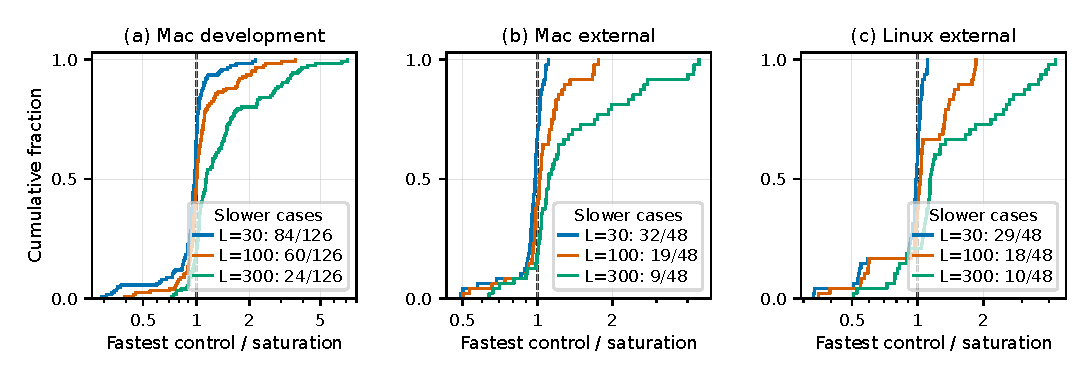
\includegraphics[width=\textwidth]{figures/saturation-cdf.pdf}
\caption{Whole-call speed ratios against the fastest measured control for
every case. The dashed line is equal runtime; values below one favor the
control. Each panel retains all three widths and reports the count of slower
candidate cases. Runs are summarized separately rather than pooled.}
\Description{Three cumulative-distribution panels for Mac development,
Mac external and Linux external, showing every width and slower-case count.}
\label{fig:saturation-cdf}
\end{figure*}

The work profiles explain a mechanism without equating work reduction with
speed. At $L=300$, aggregate saturation visits are 72.1\%, 57.5\% and
57.5\% of full-active visits, and 73.8\%, 58.3\% and 58.3\% of
last-positive visits, respectively. Median runtime ratios against the
last-positive control are 1.198, 1.136 and 1.152. Preparation, pointer
access and component bookkeeping still cost time; some cases with fewer
visits remain slower. Figure~\ref{fig:saturation-work} compares work and time
against the matched full-active control for every case; it is a descriptive
association, not an estimate of the causal cost of one visit. Seven development
series and four external series have one original interval. The theorem also
requires distinct support scores; interval count alone does not establish
its applicability.

\begin{figure*}[t]
\centering
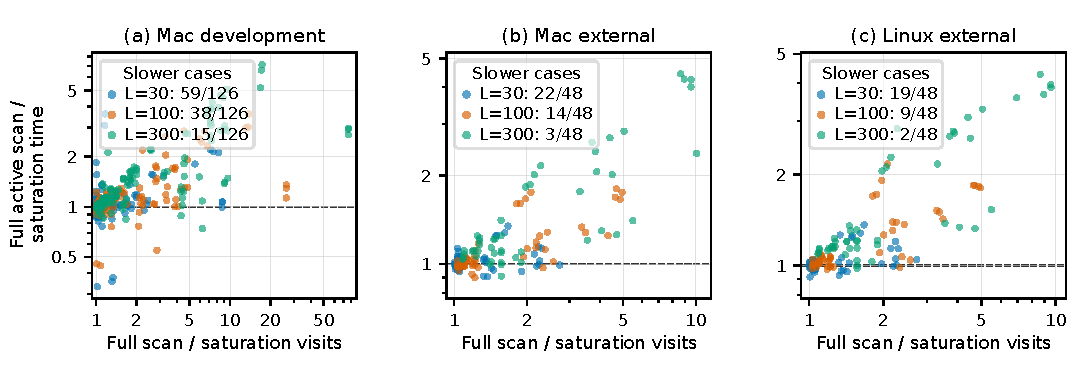
\includegraphics[width=\textwidth]{figures/saturation-work.pdf}
\caption{Traversal reduction versus full-call runtime. Horizontal position
is full-active visits divided by saturation visits; vertical position is
full-active time divided by saturation time. A work saving need
not cross the horizontal equal-runtime line. Every measured case is retained.}
\Description{Three scatter panels relate traversal reduction to complete-call
speed ratio for all cases and widths on the three study runs.}
\label{fig:saturation-work}
\end{figure*}

\subsection{Linux regeneration and additional external implementations}
The frozen Linux workflow regenerated the external inputs from pinned raw
sources, then ran the same protocol with the same source hashes. Raw data
and labels match Mac hashes. Eleven of 48 score arrays match byte for byte;
37 differ after platform-dependent scoring. This is a reproduction of the
specified input-generation procedure and evaluator experiment, not an
identical-array replay or an independent laboratory study. All 53 downloaded
artifact-file hashes were checked against the workflow manifest.

A separately frozen descriptive supplement compares the paired ROC--PR
public call against actual pinned Benchopt and DTAI implementations, with
exhaustive thresholds~\cite{benchopt2026,dtaianomaly}. It uses the 48 external
score vectors at $L=30$, three warmed complete-call repetitions, and the
released paired radix evaluator as a control. The native DTAI code retains
its parallel/fast-math compilation but runs with one compute thread.
Benchopt completes all 48 cases: its median ratio is $34.918\times$ and
the minimum is $20.079\times$. The paired radix median is only $1.017\times$,
with 19/48 candidate losses. Thus the large external-library ratio cannot
be attributed to saturation alone.

DTAI is prescribed for the Isolation Forest vector of each of the 12
series. Ten complete all repetitions; PSM and swan hit the 30-second parent
watchdog on their first timed call, and subsequent repetitions are skipped.
The two cases receive no fabricated evaluator duration or speed ratio.
The completed subset has median ratio $101.106\times$; censoring prevents
interpreting it as the median over all 12 prescribed cases. All completed
paired outputs agree within $8.22\times10^{-15}$. This supplement neither
changes the main experiment's task nor its primary decision.

\subsection{Structural mechanism checks}
A separately frozen synthetic study tests four input families at
$L\in\{32,128,512,2048\}$, with $n=4L+3$. The first places a singleton
original last among distinct scores; the second uses an eight-position
original interval with all originals last; the third realizes the
two-original separating construction, with equal middle scores below its
four decisive positions; the fourth is an all-tied singleton negative
control. All inputs, source hashes and count predictions are fixed before
timing. Each case uses three randomized warmed complete-call repetitions.
All 16 cases satisfy their count predictions and agree with released radix
within $1.39\times10^{-17}$. This comparison uses production radix rather
than an additional independent dense oracle.

The singleton distinct-score family visits $3L-1$ positions in total;
the two-original family visits $4L$. At $L=2048$, the latter visits 8,192
positions versus 4,198,402 for last-positive stopping, a $512.5\times$
traversal reduction. Its median full call takes 0.717 milliseconds, with
$17.06\times$ speedup over last-positive stopping and $53.88\times$ over
released radix. The all-tied singleton instead visits the entire active
support, as predicted. Its last-positive ratio remains close to one.
These constructed inputs demonstrate mechanisms and their limitations;
their timing gains do not estimate gains on real-world data.

\begin{table}[t]
\centering
\footnotesize
\setlength{\tabcolsep}{3.5pt}
\begin{tabular}{lrrrr}
\toprule
Family & $L=32$ & 128 & 512 & 2048\\
\midrule
Singleton, original last & 0.845 & 1.401 & 4.530 & 17.536\\
Eight originals last & 1.019 & 1.273 & 3.354 & 12.793\\
Two-original separation & 1.025 & 1.387 & 4.161 & 17.063\\
All-tied singleton & 0.972 & 1.005 & 0.998 & 1.012\\
\bottomrule
\end{tabular}
\caption{Descriptive structural-study ratios: last-positive median time
divided by saturation median time. All 16 cases are shown, including small
input overhead and the tied negative control.}
\label{tab:structural-runtime}
\end{table}

